\chapter{Filtro Hairpin}

\section*{Resumen}

En este capítulo se presenta el diseño, simulación, construcción y caracterización experimental del filtro Hairpin utilizado en la etapa de salida del sistema. El objetivo del filtro es permitir el paso de las componentes de frecuencia de interés y atenuar las componentes espectrales no deseadas generadas en las etapas anteriores. Debido a las frecuencias de operación del sistema, se seleccionó una implementación mediante líneas de transmisión microstrip, utilizando una estructura Hairpin de líneas acopladas.

\section{Introducción}

La señal obtenida a la salida del sistema puede contener, además de las componentes de frecuencia de interés, componentes espectrales no deseadas producto de las distintas etapas de procesamiento y conversión. Estas componentes pueden afectar el desempeño del sistema y deben ser atenuadas antes de entregar la señal a la siguiente etapa.

Debido a la frecuencia de operación del sistema, se optó por utilizar un filtro de microstrip en lugar de una implementación mediante componentes concentrados. Esta alternativa permite aprovechar las propiedades distribuidas de las líneas de transmisión para implementar resonadores y estructuras acopladas capaces de generar la respuesta en frecuencia requerida.

Entre las diferentes topologías de filtros de microstrip disponibles, se seleccionó la configuración Hairpin debido a su estructura compacta, facilidad de fabricación y capacidad para implementar filtros pasabanda mediante resonadores de media longitud de onda plegados. La proximidad entre los brazos de los resonadores permite establecer el acoplamiento electromagnético necesario para obtener la respuesta pasabanda.

El filtro se ubicó en la etapa de salida del sistema con el objetivo de seleccionar el intervalo de frecuencias de interés y reducir las componentes fuera de banda. Para su diseño se siguió la metodología presentada en el marco teórico, basada en el cálculo de los coeficientes del prototipo, los factores de calidad externos y los coeficientes de acoplamiento entre resonadores.

\section{Especificaciones de diseño}

El principal objetivo de este filtro es eliminar la componente de frecuencia generada durante el arranque del PLL. Esto ocurre debido a que, al encender el sistema, el valor por defecto de la tensión de control del VCO corresponde a $0~\mathrm{V}$, lo que equivale a $1350~\mathrm{MHz}$ y lleva a operar fuera de su rango previsto enviando una frecuencia no deseada a los demás componentes del radar. Como buena práctica de diseño, se busca además atenuar las componentes armónicas generadas por el propio VCO en múltiplos de la señal de interés. Por este motivo, se decide incorporar un filtro pasabanda que no interfiera con el \textit{chirp} transmitido, pero que suprima eficazmente dichas componentes fuera de banda. El diseño del filtro Hairpin se realizó con el objetivo de seleccionar la banda de frecuencias de interés y atenuar las componentes fuera de dicha banda. Las especificaciones adoptadas para el dispositivo se resumen en la Tabla~\ref{tab:especificaciones_hairpin_dev}.

\begin{table}[H]
\centering
\begin{tabular}{lc}
\hline
\textbf{Parámetro} & \textbf{Especificación} \\
\hline
Tipo de filtro & Hairpin pasabanda \\
Orden del filtro & 5 \\
Frecuencia central & $1{,}7~\mathrm{GHz}$ \\
Ancho de banda & $390~\mathrm{MHz}$ \\
Ancho de banda fraccional ($\mathrm{FBW}$) & $0{,}2294$ \\
Frecuencia inferior & $1{,}55~\mathrm{GHz}$ \\
Frecuencia superior & $1{,}85~\mathrm{GHz}$ \\
Rizado de la banda de paso & $0{,}5~\mathrm{dB}$ \\
Impedancia de referencia & $50~\Omega$ \\
Atenuación de la frecuencia $1{,}35~\mathrm{GHz}$ & $-30~\mathrm{dB}$ \\
Tecnología & Microstrip \\
Sustrato & FR-4 \\
\hline
\end{tabular}
\caption{Especificaciones de diseño del filtro Hairpin.}
\label{tab:especificaciones_hairpin_dev}
\end{table}

\section{Diseño}
Para el diseño del filtro Hairpin se seleccionó un ancho de banda fraccional de $\mathrm{FBW} = 0{,}229$ y una frecuencia central de $1{,}7~\mathrm{GHz}$. Se adoptó un prototipo pasabajos Chebyshev de quinto orden, con un rizado en la banda de paso de $0{,}5~\mathrm{dB}$. Para una frecuencia de corte pasabajos normalizada $\Omega_c = 1$, los coeficientes del prototipo son:

\begin{equation}
g_0 = g_6 = 1,
\end{equation}

\begin{equation}
g_1 = g_5 = 1{,}1468,
\end{equation}

\begin{equation}
g_2 = g_4 = 1{,}3712,
\end{equation}

\begin{equation}
g_3 = 1{,}9750.
\end{equation}

A partir de estos parámetros y del ancho de banda fraccional se calcularon los factores de calidad externos de los resonadores de entrada y salida. Para el primer resonador se obtiene:

\begin{equation}
    Q_{e1} = \frac{g_0 g_1}{\mathrm{FBW}} = \frac{(1)(1{,}1468)}{0{,}229} = 5{,}0079.
\end{equation}

Debido a la simetría del filtro, el factor de calidad externo del último resonador presenta el mismo valor:

\begin{equation}
    Q_{e5} = \frac{g_5 g_6}{\mathrm{FBW}} = \frac{(1{,}1468)(1)}{0{,}229} = 5{,}0079.
\end{equation}

Los coeficientes de acoplamiento entre resonadores consecutivos se obtuvieron mediante:

\begin{equation}
    M_{12} = \frac{\mathrm{FBW}}{\sqrt{g_1 g_2}} = \frac{0{,}229}{\sqrt{(1{,}1468)(1{,}3712)}} = 0{,}1826.
\end{equation}

\begin{equation}
    M_{23} = \frac{\mathrm{FBW}}{\sqrt{g_2 g_3}} = \frac{0{,}229}{\sqrt{(1{,}3712)(1{,}9750)}} = 0{,}1392.
\end{equation}

\begin{equation}
    M_{34} = \frac{\mathrm{FBW}}{\sqrt{g_3 g_4}} = \frac{0{,}229}{\sqrt{(1{,}9750)(1{,}3712)}} = 0{,}1392.
\end{equation}

\begin{equation}
    M_{45} = \frac{\mathrm{FBW}}{\sqrt{g_4 g_5}} = \frac{0{,}229}{\sqrt{(1{,}3712)(1{,}1468)}} = 0{,}1826.
\end{equation}

Por lo tanto, los parámetros obtenidos para el diseño del filtro son:

\begin{equation}
Q_{e1} = Q_{e5} = 5{,}0079
\end{equation}

y

\begin{equation}
M_{12} = M_{45} = 0{,}1826, \qquad M_{23} = M_{34} = 0{,}1392.
\end{equation}

Estos valores determinan las condiciones de acoplamiento que deben reproducirse mediante la geometría de los resonadores Hairpin. En particular, los diferentes valores de $M_{i,i+1}$ implican diferentes niveles de acoplamiento entre resonadores consecutivos y, por lo tanto, distintas separaciones físicas entre ellos. Sin embargo, la relación entre el coeficiente de acoplamiento y la separación no puede determinarse únicamente a partir de las ecuaciones del prototipo, ya que depende de parámetros electromagnéticos y geométricos de la estructura, como el ancho de las líneas, la longitud de los resonadores, la separación entre sus brazos, el espesor y la permitividad del sustrato. Por este motivo, siguiendo la metodología presentada en \cite{A Hasan}, las separaciones iniciales se determinaron mediante simulación electromagnética en ADS y posteriormente se optimizaron hasta obtener los coeficientes de acoplamiento requeridos. De esta manera, la geometría final del filtro se obtiene a partir de un proceso iterativo de simulación y optimización electromagnética que permite aproximar el comportamiento real de los resonadores a las condiciones establecidas por el prototipo Chebyshev.

\section{Simulación}

Una vez obtenido el diseño inicial, se implementó la estructura del filtro en el entorno de diseño de \textit{Advanced Design System} (ADS). Este software permite analizar el comportamiento electromagnético de la estructura de microstrip teniendo en cuenta las características del sustrato y la geometría de las líneas de transmisión.

En esta etapa se definieron las propiedades del material utilizado para la placa, incluyendo la permitividad relativa, el espesor del dieléctrico y el espesor del conductor. Sobre esta base se construyó la geometría del filtro Hairpin y se establecieron los puertos de entrada y salida con una impedancia característica de $50~\Omega$.

La simulación electromagnética permitió obtener los parámetros de dispersión del filtro, principalmente $S_{11}$ y $S_{21}$. El parámetro $S_{11}$ permite evaluar la adaptación del puerto de entrada, mientras que $S_{21}$ permite analizar la transmisión de la señal a través del filtro y determinar la banda de paso y la atenuación fuera de ella.

Debido a la sensibilidad del acoplamiento electromagnético respecto de las dimensiones geométricas, se realizó un proceso de ajuste de la estructura mediante el simulador electromagnético de ADS. El objetivo fue obtener la frecuencia central y el ancho de banda requeridos, procurando simultáneamente una baja pérdida de inserción dentro de la banda de paso y una adecuada atenuación de las componentes fuera de banda.

En la Figura~\ref{fig:hairpin_ads} se presenta la estructura del filtro Hairpin implementada en ADS antes de su fabricación.

\begin{figure}[H]
    \centering
    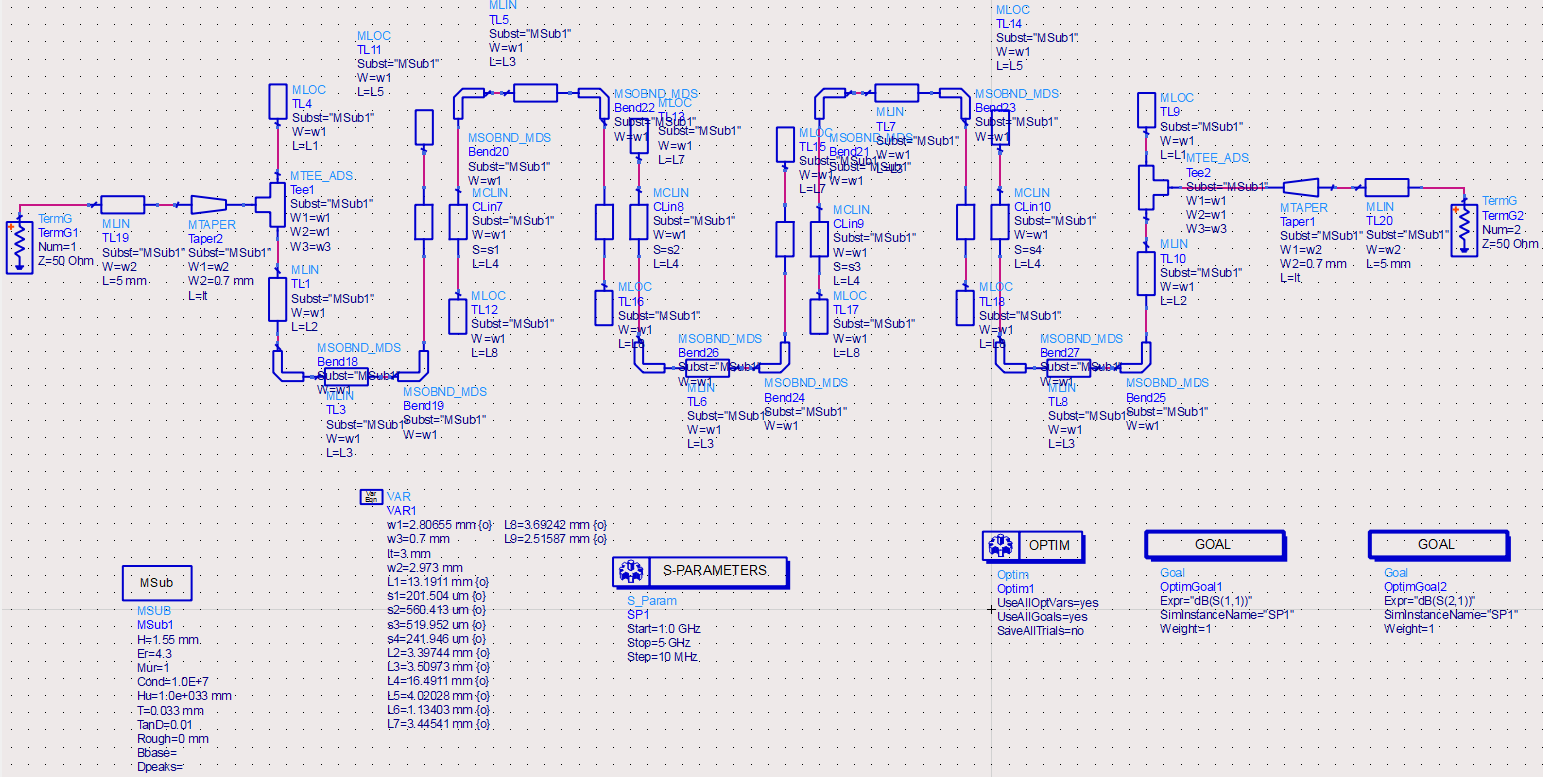
\includegraphics[width=0.85\linewidth]{imagenes/hairpin_ads.png}
    \caption{Diseño del filtro Hairpin implementado en ADS. (Fuente: propia).}
    \label{fig:hairpin_ads}
\end{figure}

El resultado de la simulación electromagnética permitió verificar que la estructura presenta el comportamiento pasabanda esperado, exhibiendo $0{,}5~\mathrm{dB}$ de rizado en la banda de interés y alcanzando una atenuación de $3~\mathrm{dB}$ para un ancho de banda de $390~\mathrm{MHz}$. En la Figura~\ref{fig:hairpin_sim} se muestran los parámetros de dispersión obtenidos mediante la simulación.

\begin{figure}[H]
    \centering
    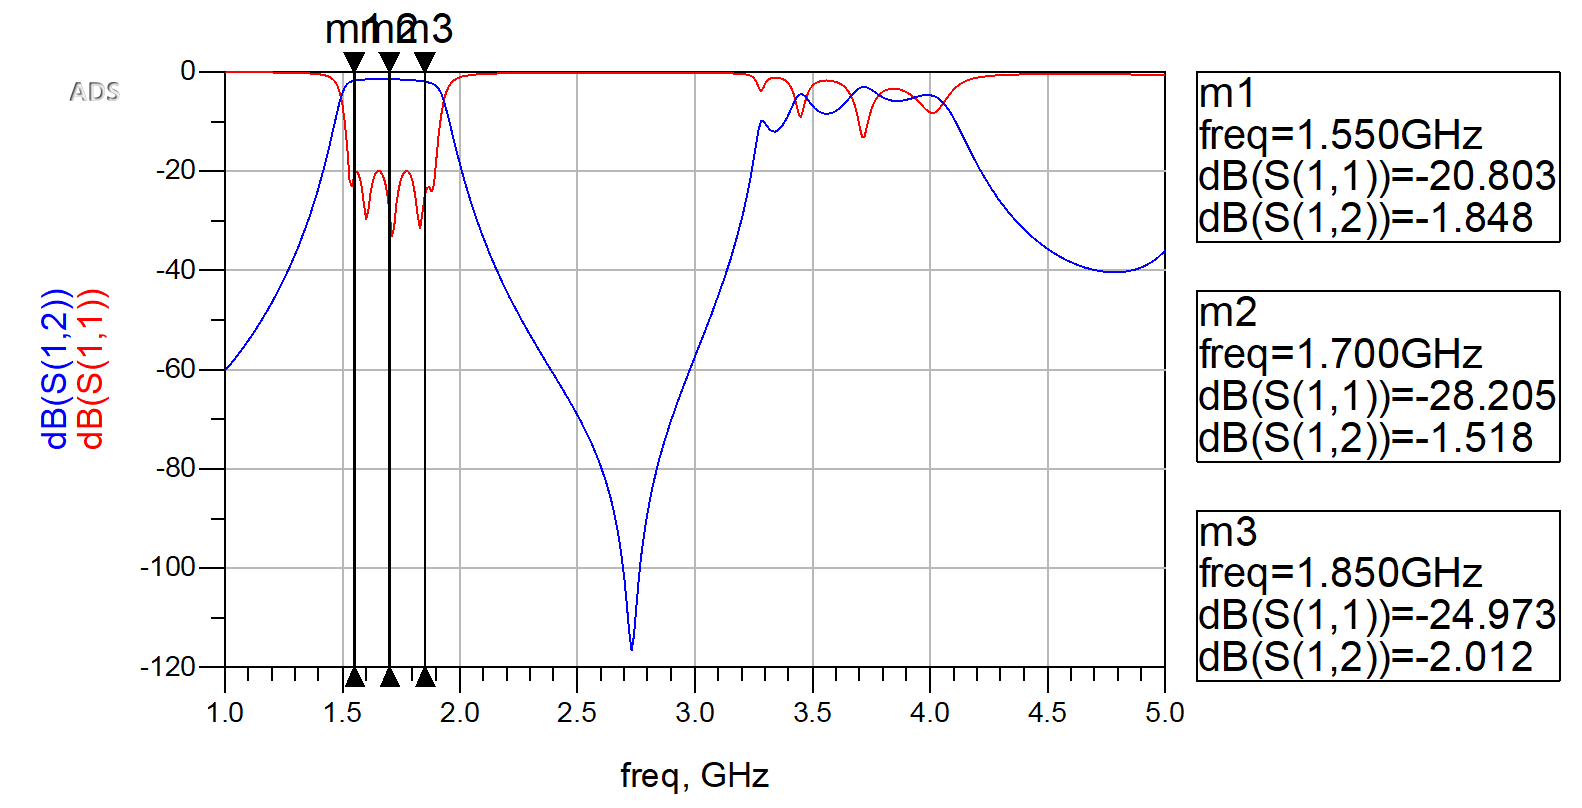
\includegraphics[width=0.85\linewidth]{imagenes/hairpin_sim.png}
    \caption{Parámetros de dispersión obtenidos mediante la simulación electromagnética del filtro Hairpin. (Fuente: propia).}
    \label{fig:hairpin_sim}
\end{figure}

Una vez realizado el proceso de simulación y optimización electromagnética, se obtuvo la geometría final del filtro Hairpin. El diseño se implementó en el entorno de \textit{Layout} de ADS, donde se definieron las dimensiones de los resonadores, las separaciones entre ellos y las líneas de entrada y salida. La disposición obtenida se muestra en la Figura~\ref{fig:hairpin_layout}, permitiendo visualizar la estructura física del filtro que posteriormente fue utilizada para la fabricación de la placa de circuito impreso.

\begin{figure}[H]
    \centering
    
\includegraphics[width=0.85\linewidth]{imagenes/hairpin_layout.png}
    \caption{Layout del filtro Hairpin obtenido mediante simulación electromagnética en ADS. (Fuente: propia).}
    \label{fig:hairpin_layout}
\end{figure}

\section{Desarrollo de la placa}

Una vez finalizado el diseño electromagnético, se procedió al desarrollo de la placa de circuito impreso. Para ello, se trasladó la geometría obtenida mediante ADS al entorno de diseño de PCB, manteniendo las dimensiones de las líneas de transmisión y la disposición de los resonadores.

La placa fue fabricada utilizando el mismo tipo de sustrato empleado en los demás bloques del sistema. Se incorporaron conectores SMA para permitir la conexión del filtro con las etapas anterior y posterior. La utilización de conectores SMA permite realizar la caracterización individual del dispositivo mediante el analizador de redes.

Los componentes utilizados se resumen en la Tabla~\ref{tab:componentes_filtro_hairpin}.

\begin{table}[H]
\centering
\begin{tabular}{lc}
\hline
\textbf{Componente} & \textbf{Característica} \\
\hline
Placa de circuito impreso & FR-4 \\
Conexión & Conectores SMA hembra \\
Acabado de PCB & Estaño líquido \\
\hline
\end{tabular}
\caption{Componentes utilizados para la construcción del filtro Hairpin.}
\label{tab:componentes_filtro_hairpin}
\end{table}

La disposición física de los conectores y de la estructura Hairpin se definió buscando mejorar la integración del filtro con los restantes módulos del sistema. Asimismo, se mantuvo la mayor correspondencia posible entre la geometría simulada y la geometría fabricada, debido a la sensibilidad de los filtros de microstrip frente a modificaciones en las dimensiones de las líneas.

Posteriormente, se realizó la fabricación de la placa y el montaje de los conectores SMA. En la Figura~\ref{fig:hairpin_fabricado} se presenta el filtro Hairpin construido.

\begin{figure}[H]
    \centering
    
\includegraphics[width=0.5\linewidth]{imagenes/hairpin_fabricado.png}
    \caption{Filtro Hairpin fabricado. (Fuente: propia).}
    \label{fig:hairpin_fabricado}
\end{figure}

\section{Mediciones}

Una vez construido el filtro, se realizó su caracterización mediante un \textit{NanoVNA} previamente calibrado. La calibración se efectuó antes de realizar las mediciones con el objetivo de reducir los errores sistemáticos introducidos por el instrumento, los cables y las conexiones utilizadas durante la medición.

El filtro fue conectado entre los dos puertos del instrumento y se realizó un barrido en el intervalo de frecuencias de interés. A partir de las mediciones se obtuvieron principalmente los parámetros $S_{11}$ y $S_{21}$, utilizados para evaluar la adaptación de entrada y la respuesta de transmisión del filtro, respectivamente.

En la Figura~\ref{fig:hairpin_medicion} se presentan los resultados obtenidos experimentalmente.

\begin{figure}[H]
    \centering
    \begin{subfigure}[b]{0.48\linewidth}
        \centering
        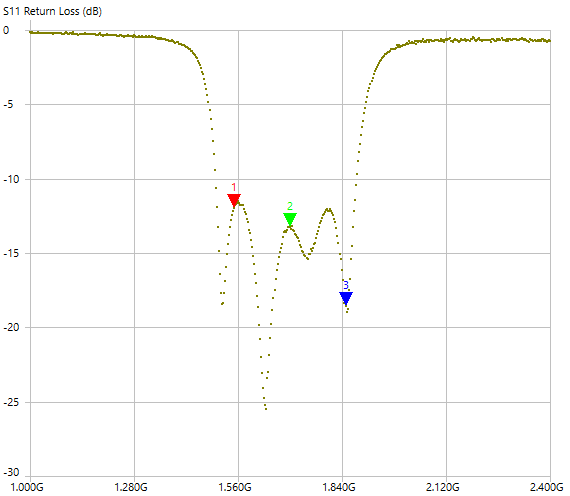
\includegraphics[width=\linewidth]{imagenes/s11.png}
        \caption{$S_{11}$ medido.}
        \label{fig:hairpin_s11}
    \end{subfigure}
    \hfill
    \begin{subfigure}[b]{0.48\linewidth}
        \centering
        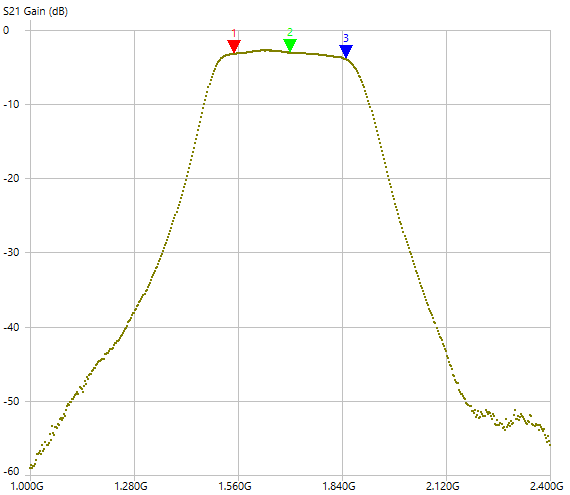
\includegraphics[width=\linewidth]{imagenes/s21.png}
        \caption{$S_{21}$ medido.}
        \label{fig:hairpin_s21}
    \end{subfigure}
    \caption{Parámetros de dispersión medidos para el filtro Hairpin. (Fuente: propia).}
    \label{fig:hairpin_medicion}
\end{figure}

Como consecuencia de las tolerancias propias del proceso de fabricación y de la elevada sensibilidad del filtro frente a las variaciones en el acoplamiento entre los resonadores, se obtuvieron pérdidas de inserción cercanas a $-12~\mathrm{dB}$ en la banda de paso. Esta sensibilidad resulta relevante debido a que la separación mínima entre resonadores en el diseño fue de apenas $0{,}4~\mathrm{mm}$, por lo que pequeñas variaciones de estas dimensiones durante el proceso de fabricación modifican el acoplamiento electromagnético entre ellos. El resultado de la medición presenta una diferencia aproximada de $8~\mathrm{dB}$ respecto del valor obtenido mediante simulación.

Por otra parte, la atenuación mínima medida en la banda de paso fue de aproximadamente $-3{,}2~\mathrm{dB}$, mientras que el resultado simulado presentó una atenuación de aproximadamente $-1{,}7~\mathrm{dB}$, obteniéndose una diferencia de $1{,}5~\mathrm{dB}$. Una de las principales fuentes de discrepancia entre los resultados simulados y experimentales corresponde a las propiedades reales del sustrato empleado. El material utilizado para la fabricación del filtro no contaba con una hoja de datos que proporcionara los valores medidos de permitividad relativa y tangente de pérdidas a la frecuencia de operación.

La última diferencia se encuentra en el rizado medido, que fue de $0{,}8~\mathrm{dB}$ comparado con los $0{,}5~\mathrm{dB}$ de la simulación (valor aceptable para la aplicación), y un desplazamiento del ancho de banda a $3~\mathrm{dB}$ de $5~\mathrm{MHz}$.